\documentclass{article}
\usepackage[utf8]{inputenc}
\usepackage{float}
\usepackage[english]{babel}
\usepackage{authblk}
\usepackage{natbib}
\usepackage[export]{adjustbox}% http://ctan.org/pkg/adjustbox
\usepackage{subfiles}
\usepackage{mathtools}
\usepackage{xurl}
\usepackage{pdflscape}
\usepackage{graphicx}
\usepackage{tikz}
\usepackage{lineno}
\usepackage{adjustbox}
\usepackage{setspace}
\usepackage{dsfont}
\begin{document}
\title{A simple test to uncover signals of CpG hypermutability using posterior predictive simulations}
\author[1]{Simon Laurin-Lemay}
\author[1,2,3]{Nicolas Rodrigue}
\affil[1]{Department of Biology, Carleton University, Ottawa, Canada}
\affil[2]{Institute of Biochemistry, Carleton University, Ottawa, Canada}
\affil[3]{School of Mathematics and Statistics, Carleton University, Ottawa, Canada}
\date{}
\maketitle
\section*{Keywords}
DNA sequence evolution, Markov chain Monte Carlo, phylogenetics, misspecification, confounding factors
\section*{Declarations}
Conflict of interest: The authors declare that they have no competing
interests.
\section*{Correspondence}
Simon Laurin-Lemay\\
209 Nesbitt Biology Building,\\
1125 Colonel By Drive Ottawa,\\
Ontario, CANADA\\
K1A 0C6\\
evol.simon@gmail.com\\
% tel: +1 613 520 2600 x 41941\\
\clearpage
\doublespacing

\section*{Abstract}
\subsection*{Objective}
CpG hypermutability is a process known to impact vertebrate evolution and is caused by spontaneous deamination of methylated cytosines within CpG contexts.  CpG hypermutability has been shown to confound the detection of negative and positive selection on codon usage and amino acids.  In this work, we propose a simple test based on the use of posterior predictive sampling to detect the presence of CpG hypermutability using the GTR+G substitution model.

\subsection*{Results}
First, we validated the CpG test using simulations. We recovered between 0-8\% of false positives and no false negatives. The simulations were performed using the jump-chain algorithm with a simple codon substitution model for more realistic simulation conditions and to allow for different degree of CpG hypermutability. All mammalian genes tested were positive with the posterior predictive test we developed to detect CpG hypermutability, which is consistent with previous results obtained using complex mechanistic phylogenetic codon substitution models designed to measure the level of CpG transition rate.  This test could easily accompany any study aimed at detecting negative or positive selection, even for large-scale analyses, knowing that methylation of cytosines exists in all domains of life (i.e., bacteria, archaebacteria, and eukaryota).

\clearpage
\linenumbers
\section*{Introduction}
The phylogenetic method involves first the generation of data sets and then the analysis of those data sets with various substitution models.  This is followed by a cycle of work in which molecular evolutionists compare measurements of population processes (i.e. mutation, selection, even demographic processes) included in the definitions of their models \citep[e.g.][]{Rodrigue2020,Latrille2021a}.  One of the things most feared by molecular evolutionists is the discovery of confounding effects \citep[e.g.,][]{LaurinLemay2018a,LaurinLemay2022} which could invalidate the proposed mechanistic hypothesis testing approach to detect and measure levels of specific evolutionary processes.  Confounders are evolutionary processes not accounted for by the substitution model.  In the Bayesian framework, the presence of confounders will incorrectly affect the posterior values of one or more parameters of the substitution model, which was designed to parameterize another population process.  Finally, false positives can result from the presence of confounders.  For example, the hypermutability of CpGs due to the process of spontaneous deamination of methylated cytosines in CpG contexts may confound the detection of negative or positive selection on synonymous and non-synonymous mutations \citep[e.g.,][]{LaurinLemay2018a,LaurinLemay2022}.

Once a confounding process has been identified, researchers should go back to the original data sets and try to control for that aspect, if possible, by removing the sites affected by the confounding process: \citep[e.g.,][]{Dunn2019}.  On the other hand, managing confounders by selecting sites for analysis may be particularly difficult or even impossible when dealing with confounders that affect substitution processes with dependencies between sites, such as the hypermutability of CpGs.  Ultimately, the researcher should propose ways to incorporate the confounding process into a new substitution model, so that the process can be conditioned jointly with other evolutionary processes, or in a two-step procedure (e.g., topology is usually not co-conditioned with other mutation and selection parameters in the field of molecular evolution).

Most substitution models assume that sites evolve independently, which is particularly convenient for calculating the likelihood of an alignment; we only need to multiply all the site likelihoods calculated from each site of the alignment \citep{Felsenstein1981}.  On the other hand, taking into account substitution processes involving dependencies between sites \citep[e.g.,][]{Robinson2003,Rodrigue2005,LaurinLemay2018b,Meyer2019}, as required to parameterize the hypermutability of CpGs, is not a trivial task.  Dealing with such substitution processes makes the development of mathematics and code more complex and limited to a small circle of researchers. This has led researchers to develop hybrid methods that integrate standard posterior sampling methods (e.g., Markov Chain Monte Carlo) with so-called simulation-based methods \citep[e.g.,][]{LaurinLemay2018b} or to develop strategies that rely on data augmentation \citep[e.g.,][]{Robinson2003,Rodrigue2005}.

Posterior predictive sampling \citep{Gelman1996,Brown2018} is a central tool in the Bayesian toolbox. This tool is of primary use when validating new phylogenetic models \citep[e.g.,][]{Huelsenbeck2001,Brown2014}.  For example, knowing that CpGs are depleted by the high rate of spontaneous deamination due to methylation of most vertebrate cytosines within CpG contexts \citep{Bird1980,Burge1992}, we are interested in the ability of substitution models to predict dinucleotide (e.g. CpG) frequencies of mammalian protein-coding genes.

Following the textbook case of mammalian CpG hypermutability, we will test our ability to detect the presence of CpG hypermutability using one of the most widely used substitution models, the GTR+G substitution model, using Bayesian posterior predictive sampling.  By definition, we expect the GTR+G substitution model to predict more CpG dinucleotides than would be observed in real alignments because CpG hypermutability is not accounted for in the model definition.  Similarly, the GTR+G substitution model will allow stop codons to be generated within predictive alignments.  We first validated the posterior predictive test using simulations generated without and with CpG hypermutability, using the GTR+G substitution model and a codon substitution model implemented in the mutation selection framework.  The codon substitution model used uses a GTR parameterization for the background mutation process plus a $\lambda$ parameter for CpG hypermutability and a parameter to capture global negative selection on amino acids.  We then apply the test to 137 mammalian protein-coding genes for which we have already measured the degree of CpG hypermutability using a complex codon substitution model \citep{LaurinLemay2018b}. Finally, we discuss the ranking of other dinucleotides in terms of their ability to be predicted by the GTR+G substitution model using the same approach developed for testing for the presence of CpG hypermutability.

\section*{Materials and methods}
\subsection*{Detecting CpG hypermutability using posterior predictive sampling}
The CpG test consists of calculating the proportion of times, i.e., \emph{p-value}, that the frequency of CpGs calculated from the real alignments is lower than the CpG frequency recovered from the predictive alignments, where the predictive alignments are generated from a set of parameter values, $i$, sampled from the posterior.  The following equation details the CpG test:

\begin{equation}\label{test}
 \text{\emph{p-value}} = \frac{1}{N}\sum_{i=1}^{N}1(freq_{CpG}^{real}<freq_{CpG}^{pred_{i}}),
\end{equation}

where $N$ is the predictive sample size and $1$ is an indicator function that returns 1 if the CpG frequency calculated from the true alignment is less than the predictive CpG frequency and 0 otherwise.

\subsection*{Real data and tree topology}
We retrieved the 137 mammalian codon alignments from \citet{LaurinLemay2018a} along with the tree topology.

\subsection*{Simulation study}
We first analyzed 10 mammalian protein-coding genes selected for their wide range of GC content as used to validate the new approach developed in \citet{LaurinLemay2018b} using the GTR+G substitution model as well as the M0GTR codon substitution model, but with $\omega$ fixed at 1 \citep{Yang2000} using Phylobayes-MPI \citep{Lartillot2013} ** jai fait une petite bourde ici, en laissant omega fixed, mais c'est juste pour avoir des valeurs de paramètres, donc ca ne dérange pas **.  We generated 100 predictive alignments (10 genes $\times$ 10 samples) using AliSim \citep{LyTrong2022} for the GTR+G substitution model, which will later be analyzed with the same model to generate a new set of predictive alignments on which to apply the CpG test.  We also generated 600 predictive alignments (10 genes $\times$ 3 values of $\lambda$ $\times$ 2 values of $\omega$ $\times$ 10 posterior predictive samples) under the M0GTR substitution model using the jump chain simulation algorithm described in \citet{LaurinLemay2022} to account for CpG hypermutability. All simulations were performed with a single $\omega$ value (i.e., 0.2 or 1). To evaluate the false positive and false negative rates of the test, we generated predictive alignments using $\lambda = 1$ and $\lambda = \{4.8\}$, respectively.

Each simulated predictive alignment was then analyzed with the GTR+G substitution model using Phylobayes-MPI \citep{Lartillot2013} software, we generate posterior predictive alignments, 50 for each analysis, using the same software.  The predictive alignments were generated by sampling 50 sets of parameter values from the posterior of each of the GTR+G analyses performed on synthetic alignments. Each of the experimental conditions (3 values of $\lambda$ $\times$ 2 values of $\omega$) is replicated 100 times.  The proportion of false positives and false negatives in each set of experimental conditions was then calculated by applying the posterior predictive tests.

\subsection*{Empirical study}
We analyzed the 137 mammalian codon sequence alignments with the GTR+G substitution model implemented in Phylobayes-MPI: \citep{Lartillot2013}.  We sample 100 posterior predictive alignments, also using Phylobayes-MPI, for each mammalian gene of interest.  We then apply the posterior predictive test by calculating the frequency of CpGs from the true and predictive alignments to detect the presence of CpG hypermutability. Similarly, for each dinucleotide context, we could apply the specific predictive test as designed for the CpG context and calculate the proportion of positive tests to identify dinucleotide contexts missed by the GTR+G substitution model.

\section*{Results}
\subsection*{Simulation study}
Less than 5\% of the CpG tests were significant when performed on synthetic sequence alignments generated under the GTR+G substitution model, i.e., 2\% (Table \ref{table_1}).  Similarly, none of the CpG tests were significant when performed on synthetic sequence alignments generated without CpG hypermutability and with $\omega = 0.2$ using the M0GTR codon substitution model (Table \ref{table_1}). On the other hand, under less realistic conditions, without negative selection on amino acids, $\omega=1$, we recovered more false positives, i.e., 8\% (Table \ref{table_1}), but still close to the alpha significance threshold of 5\%. No false negatives were generated in the presence of CpG hypermutability, (i.e., Table \ref{table_1}: $\lambda = \{4,8\}$), all CpG tests were positive, for both of the omega values used, i.e., $\omega = \{0.2, 1\}$.

\subsection*{Empirical study}
Therefore, after validating the CpG test, we analyzed 137 mammalian protein-coding genes with the GTR+G substitution model and found 100\% of the tested genes to be significant (\emph{p-value}=0, $\alpha$=5\%), rejecting the null hypothesis that the GTR+G substitution model accounts for CpG hypermutability.  In other words, CpG frequencies are significantly reduced in all real alignments compared to frequencies recovered from predicted alignments generated by the GTR+G substitution model. As an example, in Figure 1, panel A, we show the discrepancy between the CpG frequencies predicted by the GTR+G substitution model and the observed CpG frequency in one of the examined coding sequence alignments. In panel B of the same figure, we see that the predicted values of ApT are distributed on either side of the actual value calculated from the same gene examined in panel A.

Next, we applied the predictive test to all other dinucleotide contexts using the same substitution model, i.e., GTR+G. After CpG, TpA, and GpT contexts, it was found that the GTR+G substitution model significantly missed most of the tested genes (94.9\% and 81\%, respectively; Table S1), considering an alpha significance threshold of 5\%.

\section*{Discussion}
In this work, we designed a simple test, based on posterior predictive sampling, a tool from the Bayesian toolbox, to detect the presence of CpG hypermutability. We validated the test using a simulation study: with approximately the alpha significance threshold of false positives and no false negatives. We then applied the test to a set of mammalian protein-coding genes, for which we had already obtained measurements of CpG hypermutability using a complex codon substitution model implemented in the mechanistic mutation-selection framework \citep{LaurinLemay2018b}.

We also showed that contexts other than CpG were systematically missed by the predictive samples generated by the GTR+G substitution model, namely TpA with 94.9\% of genes detected as positive (Table S1) and GpT with 81\% of positive tests (Table S1). The TpA context may be artifactually overpredicted by the GTR+G substitution model because it does not take into account the structure of the genetic code and allows the presence of stop codons in predictive protein-coding sequence alignments. Two out of three stop codons contain a TpA dinucleotide (i.e., TAA and TAG). The use of a codon substitution model implemented in the mechanistic mutation-selection framework, such as the one used here to validate the CpG test, i.e., M0GTR, should at least help to reduce the over-prediction of TpA contexts by disallowing the presence of stop codons within the predictive alignments generated when running the test, as the substitution model imposes infinite negative selection against mutations that land on stop codons. On the other hand, the etiology of TpA context depletion is highly controversial and may not be exclusively due to mutation or selection processes \citep[e.g.,][]{Duret2000,Simmonds2013}.  Interestingly, GpT contexts have been shown to be hypermutable on shorter evolutionary timescales, i.e. within human populations \citep{Simmonds2013}, suggesting that the evolutionary process behind the depletion of GpT context is conserved over the mammalian tree.  On the other hand, considering contexts other than CpG should also require extending the scope of the simulation study, since predicting the effect of one mutation process on another mutation process is particularly complicated. For example, CpG and TpA contexts share the same transition products (TpG and CpA).

However, knowing that CpG hypermutability could affect the measurement of negative and positive selection on synonymous and nonsynonymous mutations \citep{LaurinLemay2018a,LaurinLemay2022}, the test could be systematically applied when conducting large-scale evolutionary studies \citep[e.g.,][]{Murrell2015,Davydov2019,Slodkowicz2020} or in future projects such as the Zoonomia Project \citep{Zoonomia2020} to promte the development of new mechanistic tests using codon substitution models that take into account a wider range of population processes \citep[e.g.,][]{Rodrigue2010b,Lartillot2012,Rodrigue2017,LaurinLemay2018b,Rodrigue2020,Latrille2021a}. We could also investigate the presence of hypermutability patterns from substitution mappings, similar to what has been developed by \citep{Nielsen2002,Bollback2005}.

\section*{Limitations}
The main limitation of this study is that we have not yet investigated how a non-mechanistic test, such as the one developed here based on comparison of posterior predictive alignments, might be affected by the presence of other population processes (i.e. mutation, selection, and demographic processes) not accounted for by the GTR+G substitution model, which could be addressed by simulation studies. Because the CpG test we developed here is non-mechanistic, it also does not allow quantification of the degree of CpG hypermutability, as a proper mechanistic test could do \citep[e.g.,][]{LaurinLemay2018b}.

\section*{Availability of data and materials}
Workflow and data is available.

\section*{Abbreviations}


\newpage
\section*{Figures}

\begin{figure}[H]
  \centering
  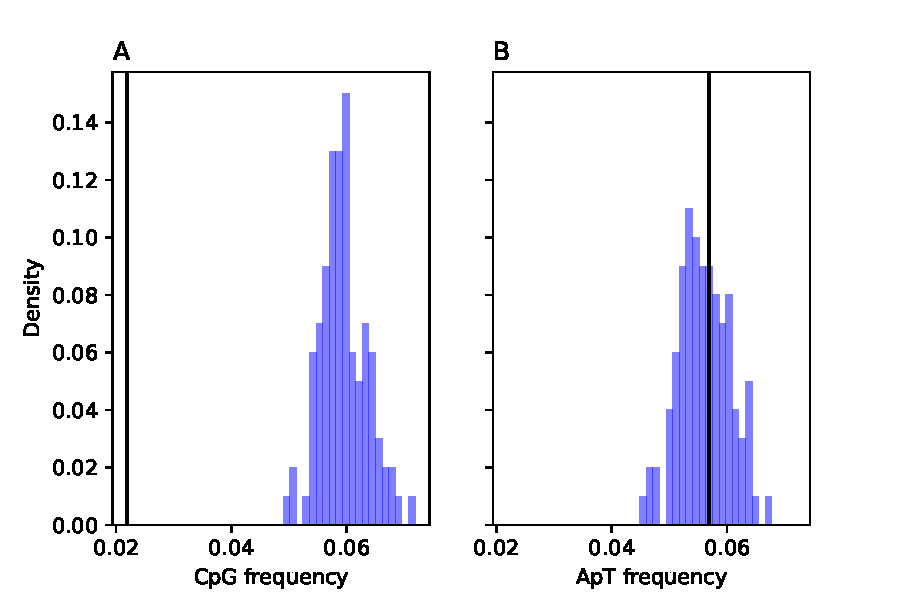
\includegraphics[width=\textwidth,height=\textheight,keepaspectratio]{figures/figure1.pdf}
  \caption{Comparison of CpG (A) and ApT (B) frequencies computed from the \emph{MEP1A} mammalian protein-coding gene alignment, black vertical lines, and corresponding frequencies computed from posterior predictive alignments generated using the GTR+G substitution model, blue histograms. Note that the predicted CpG frequencies (A) overestimate the true value 100\% of the time, while the true ApT frequency (B) falls within the distribution of predicted frequencies.}
  \label{figure1}
\end{figure}

\newpage
%\begin{landscape}
\section*{Tables}

\begin{table*}[h]
    \begin{tabular}{cccccc}
    type of controls & models used to generate the synthetic alignments & positive tests (\%)\\
    \hline
    negative & GTR+G                              & 0\\
    negative & M0GTR+($\lambda=1$)+($\omega=0.2$) & 0\\
    negative & M0GTR+($\lambda=1$)+($\omega=1.0$) & 8\\
    positive & M0GTR+($\lambda=4$)+($\omega=0.2$) & 100\\
    positive & M0GTR+($\lambda=4$)+($\omega=1.0$) & 100\\
    positive & M0GTR+($\lambda=8$)+($\omega=0.2$) & 100\\
    positive & M0GTR+($\lambda=8$)+($\omega=1.0$) & 100\\
    \hline
    \end{tabular}
    \caption{Validation of CpG test using posterior predictive sampling under GTR+G substitution model with an $\alpha$ threshold of significance 5\%. Synthetic alignments were generated using GTR+G and M0GTR codon substitution model using three CpG hypermutabilities values, $\lambda = \{1,4,8\}$ and a global selection on amino acids using two $\omega$ values (i.e., 0.2 and 1).}\label{table_1}
\end{table*}
%\end{landscape}
\newpage
\bibliographystyle{spbasic}
\bibliography{refs/refs}
\newpage
\section*{Acknowledgments}
This work was funded by the Natural Sciences and Engineering Research Council of Canada.
\section*{Funding}
\section*{Author information}
\subsection*{Authors and Affiliations}
\subsection*{Contributions}
Conceptualization: SLL, NR. Formal analysis: SLL Investigation: SLL, NR. Methodology: SLL, NR. Resources: SLL, NR. Supervision: NR Writing original draft: SLL, NR. Review and editing: SLL, NR. \\
All authors read and approved the final manuscript.
\subsection*{Corresponding author}
Correspondance to Simon Laurin-Lemay
\section*{Ethics declarations}
\subsection*{Ethics approval and consent to participate}
Not applicable.
\subsection*{Consent for publication}
Not applicable.
\subsection*{Competing interests}
The authors declare that they have no competing interests.
\subsection*{Additional information}
\section*{Supplementary information}
Table S1: Proportion of positive tests calculated for each dinucleotide context obtained using GTR+G substitution model over the 137 mammalian protein-coding genes studied.
\end{document}
